\begin{frame}{PRIME+PROBE}
    \begin{itemize}
    \item name in literature: PRIME + PROBE
    \item PRIME: fill cache (or part of it) with values
    \item do thing that uses cache
    \item PROBE: access those values again and see if it's slow
    \vspace{.5cm}
    \item coined in attacks on AES encryption
    \end{itemize}
\end{frame}

\begin{frame}{example: AES (1)}
\begin{itemize}
\item from Osvik, Shamir, and Tromer, ``Cache Attacks and Countermeasures: the Case of AES'' (2004)
\item early AES implementation used lookup table
\item goal: detect index into lookup table
    \begin{itemize}
    \item index depended on key + data being encrypted
    \end{itemize}
\item tricks they did to make this work
    \begin{itemize}
    \item vary data being encrypted
    \item subtract average time to look for what changes
    \item lots of measurements
    \end{itemize}
\end{itemize}
\end{frame}

\begin{frame}{example: AES (2)}
\small from Osvik, Shamir, and Tromer, ``Cache Attacks and Countermeasures: the Case of AES'' (2004) \\
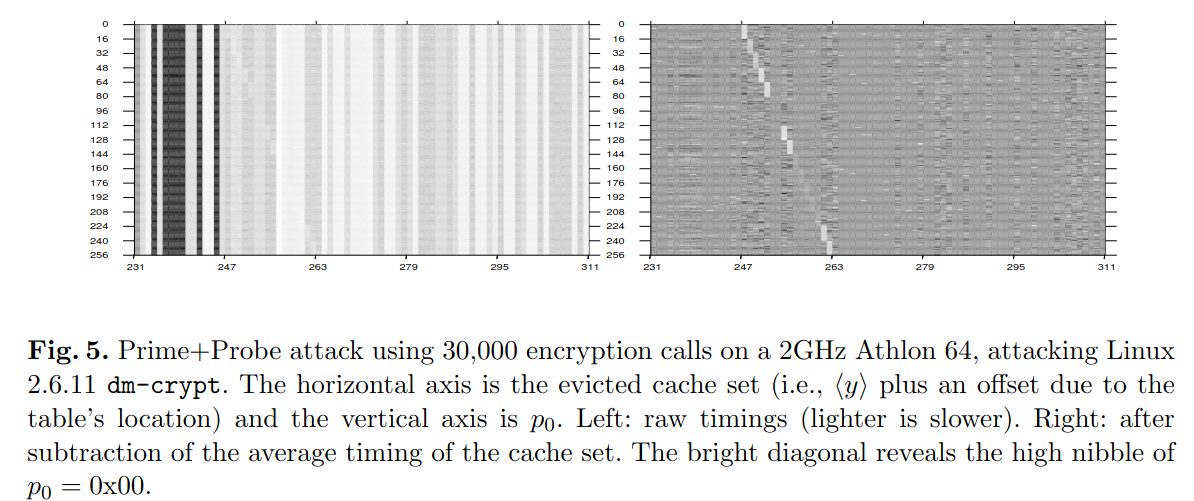
\includegraphics[width=1.0\textwidth]{../spectre/prime-probe-osvik}
\end{frame}
